\documentclass[conference]{IEEEtran}

\usepackage[utf8]{inputenc}
\usepackage[T1]{fontenc}
\usepackage{silence}\WarningsOff[latexfont]

\usepackage{listings}

\usepackage{amsmath}
\usepackage{dsfont}
\usepackage{amssymb}

\RequirePackage{tikz}[2010/10/13]
\usetikzlibrary{arrows,automata,calc,intersections,patterns,decorations.pathmorphing,decorations.pathreplacing}

\usepackage{graphicx}
\usepackage{cite}
\usepackage{url}
\usepackage[caption=false,font=footnotesize]{subfig}
\usepackage[binary-units,per-mode=symbol]{siunitx}
\sisetup{list-final-separator = {, and }}
\usepackage{booktabs}
\usepackage{pifont}
\usepackage{microtype}
\usepackage{textcomp}
\usepackage[american]{babel}
\usepackage[noabbrev,capitalise]{cleveref}
\usepackage{xspace}
\usepackage{hyphenat}
\usepackage{bm}
\usepackage[draft,inline,nomargin,index]{fixme}
\fxsetup{theme=color}
\usepackage{grffile}
\usepackage{xfrac}
\usepackage{multirow}
\RequirePackage{xstring}
\RequirePackage{xparse}
\RequirePackage[index=true]{acro}
\NewDocumentCommand\acrodef{mO{#1}mG{}}{\DeclareAcronym{#1}{short={#2}, long={#3}, #4}}
\NewDocumentCommand\acused{m}{\acuse{#1}}
\usepackage{upquote}

% TODO: remove this
\acrodef{WSN}{Wireless Sensor Network}
\acrodef{MANET}{Mobile Ad Hoc Network}
\acrodef{ROI}{Region of Interest}{short-indefinite={an}, long-plural-form={Regions of Interest}}

\begin{document}

\title{
    Rosenblatt Perceptron\\
    \large Neural Networks and Computational Intelligence - Practical Assignment I
}

\author{
    \IEEEauthorblockN{Samuel Giacomelli}
    \IEEEauthorblockA{\small Student Number: S3546330 \\ s.giacomelli@student.rug.nl}
    \and
    \IEEEauthorblockN{Davide Pedranz}
    \IEEEauthorblockA{\small Student Number: S3543757 \\ d.pedranz@student.rug.nl}
}

\maketitle

\begin{abstract}
    Rosenblatt perceptrons are powerful devices able to learn a linear boundary in a binary classification problem.
    In this assignment, we implement and train and a Rosenblatt perceptron on random generated data.
    We use the results of multiple simulations to estimated the capacity of the hyperplane defined by the learned weights.
\end{abstract}

\acresetall

\section{Introduction}
\label{sec:introduction}

Perceptrons are devices used to solve binary classification problems.
A perceptron tries to learn a hyperplane that divides the training examples in $2$ groups, depending on their label.
In general, if the dataset is linear separable, there is an infinite number of hyperplanes that perfectly separates the examples based on their labels.
The MinOver algorithm \cite{minover} tries to find the hyperplane with the maximum stability, i.e. maximize the distance of the closest examples from the hyperplane.

In this assignment, we implement the MinOver training algorithm and measured its generalization error on a linearly separable dataset as a function of the rate between the number of examples and their dimension.
We also compare its performances with the Rosenblatt algorithm \cite{rosenblatt} implemented in the previous assignment.
Finally, we introduce different degrees of noise in the datasets and observe the performances of both algorithms.

\cref{sec:theory} introduces the MinOver training algorithm.
\cref{sec:implementation} describes the implementation of the various experiments.
\cref{sec:evaluation} discusses the obtained results.
Finally, \cref{sec:conclusion} summarizes the most interesting results.

\section{Theory}
\label{sec:theory}

This time the focus was to find the perceptron of \textbf{maximum stability}, which means trying to maximize the margin between the
weight vector and the closest input label, or in other words trying to approximate to the teacher perceptron $\bm{\mathsf{w}}^*$.
The stability is therefore defined exactly as the distance mentioned former using the formula [\ref{eq:perceptron-stability}].

The dataset used is slightly different from the one of the Rosenblatt algorithm and the difference consists in defining the labels
as the sign of the dot product between the input and the vector that represents the teacher perceptron (i.e. the result of the
classification performed by the teacher perceptron for each input) (Formula [\ref{eq:labels_definition}]). 

The stability is calculated for every input vector contained in the dataset and, after finding all the values of $\kappa$,
the minimum is searched (Formula [\ref{eq:minimum_lookup}]) and a Hebbian update (Formula [\ref{eq:hebbian_update}]) is performed using the input vector
respect to that the perceptron has the minimum stability, the in order to maximize the value of that property.

This procedure is iterated over the number of epochs $n_{max}$ and stopped before reaching that value just if the last update
corresponds to a zero update (i.e. $\bm{\mathsf{w}}(t+1) = \bm{\mathsf{w}}(t)$). 

\begin{equation} \label{eq:labels_definition}
    S^\mu = sign(\bm{\mathsf{w}} \cdotp \xi^\mu)
\end{equation}

\begin{equation} \label{eq:perceptron-stability}
    \kappa^\mu = \frac{\bm{\mathsf{w}} \cdotp \xi^\mu S^\mu_R}{\lvert \bm{\mathsf{w}} \rvert}
\end{equation}

\begin{equation} \label{eq:minimum_lookup}
    \kappa^{\mu(t)} = \min_\nu \left \{ \kappa^{\nu(t)} =  \frac{\bm{\mathsf{w}} \cdotp \xi^\mu S^\mu_R}{\lvert \bm{\mathsf{w}} \rvert} \right \}
\end{equation}

\begin{equation} \label{eq:hebbian_update}
    \bm{\mathsf{w}}(t+1) = \bm{\mathsf{w}}(t) + \frac{1}{N} \xi^{\mu(t)} S^{\mu(t)}_R
\end{equation}
\section{Implementation}
\label{sec:implementation}

\subsection{Training and Test Set}
In different experiments we use a different number of training examples.
Given the original dataset $\mathbb{D} = \{ \varepsilon_\mu, \tau(\varepsilon_\mu)\}_{\mu=1}^M$ (with $M = 5000$), we create the training $\mathbb{D}_{train}$ and test set $\mathbb{D}_{test}$ as follows:
\begin{equation*}
    \begin{split}
        \mathbb{D}_{train} &= \{ \varepsilon_\mu, \tau(\varepsilon_\mu)\}_{\mu=1}^P, \\
        \mathbb{D}_{test} &= \{ \varepsilon_\mu, \tau(\varepsilon_\mu)\}_{\mu=Q}^M,
    \end{split}
\end{equation*}
with $Q > P$.
Since we choose $P \in [1, 2000]$ in different experiments, we fix $Q = 2001$ for all experiments, in order to always test on the same dataset. 

\subsection{Stochastic Gradient Descent}
The first step of our implementation of Stochastic Gradient Descent is to initialize the weights' vectors with random values and then normalize them to have unit norm $||w_j|| = 1$.
It is important to initialize the weights randomly in order to avoid symmetry problems:
since the weights gradient and the update rule is the same for all hidden unit, the updates at each epoch are also the same, which causes all units to learn the same final weights and reduces the representation power of the network.
Then, we perform a given number of updates:
at each iteration, we randomly select an example $\nu$ from the training dataset, compute the gradient with respect to the weights (see \cref{sub:gradients}) and update them according to \cref{eq:weights-update}.

At regular intervals (i.e. after a fixed number of iterations), we compute the error on both the entire training and the test sets, as shown in \cref{eq:cost-total}.

\section{Evaluation}
\label{sec:evaluation}
If not differently specified, all experiments discussed in this section are run with the following parameters: $N = 500$, $n_{max} = 200$, $n_D = 100$ and $c = 0$.

\subsection{Storage Capacity}
\label{subsec:capacity}
\begin{figure}[t]
	\centering
	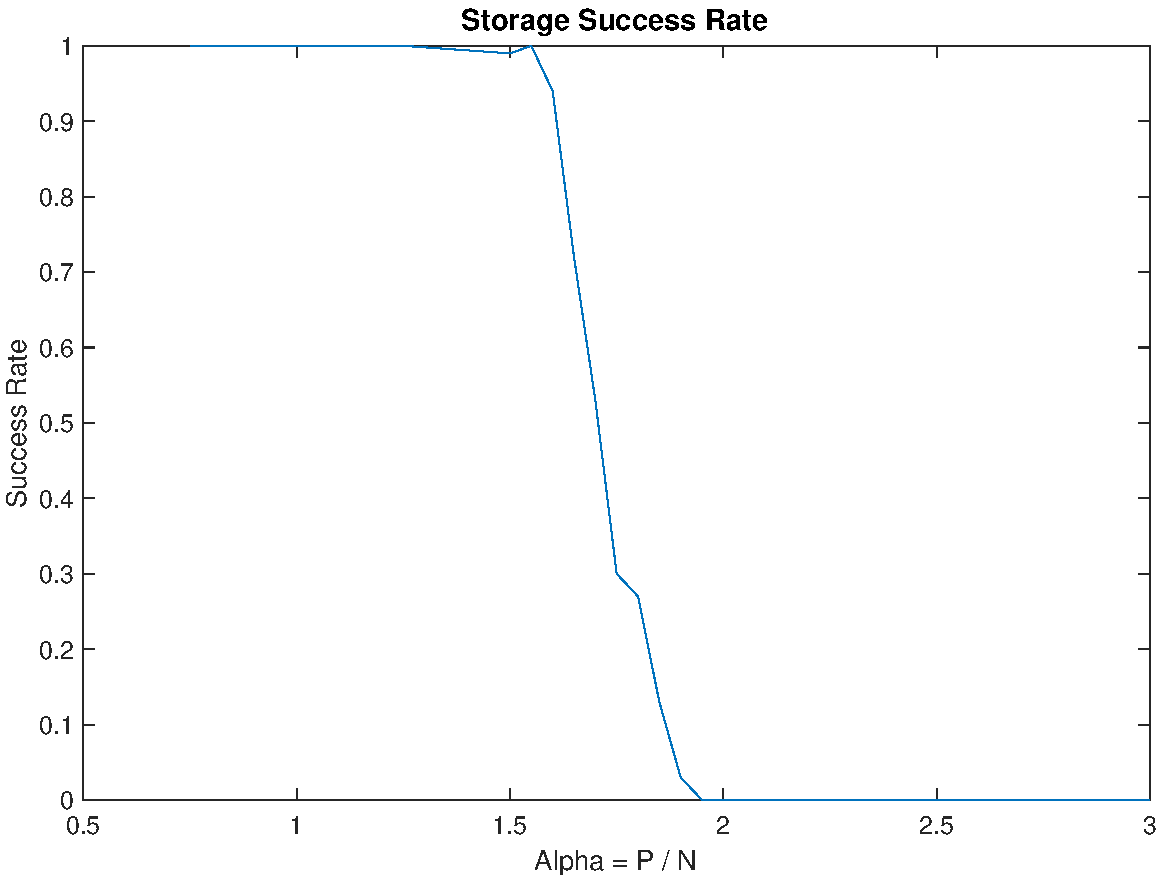
\includegraphics[width=\columnwidth]{figures/base}
    \caption{Storage success rate of a Rosenblatt perceptron as a function of $\alpha = P / N$. The experiments use $N = 500$, $n_{max} = 200$ and $n_D = 100$.}
	\label{fig:base}
\end{figure}
\cref{fig:base} shows the results of the base experiment.
The x-axis represent different values of $\alpha = P / N$, while the y-axis the success rate $Q_{l.s.}$.
As expected, the function looks like a step function from $1$ to $0$.
For $\alpha \approx 1.7$, the success rate $Q_{l.s.}$ drops from $1$ to $0$ very quickly. 

The value of $\alpha$ for which the function drops is called storage capacity of the perceptron.
For $N \to \infty$ (very large number of examples) and $n_{max} \to \infty$ (no limit on the maximum number of training iterations), the theoretical storage capacity of the Rosenblatt perceptron is $\alpha = 2$.

\subsection{Number of Iterations}
\label{subsec:epochs}
\begin{figure}[t]
	\centering
	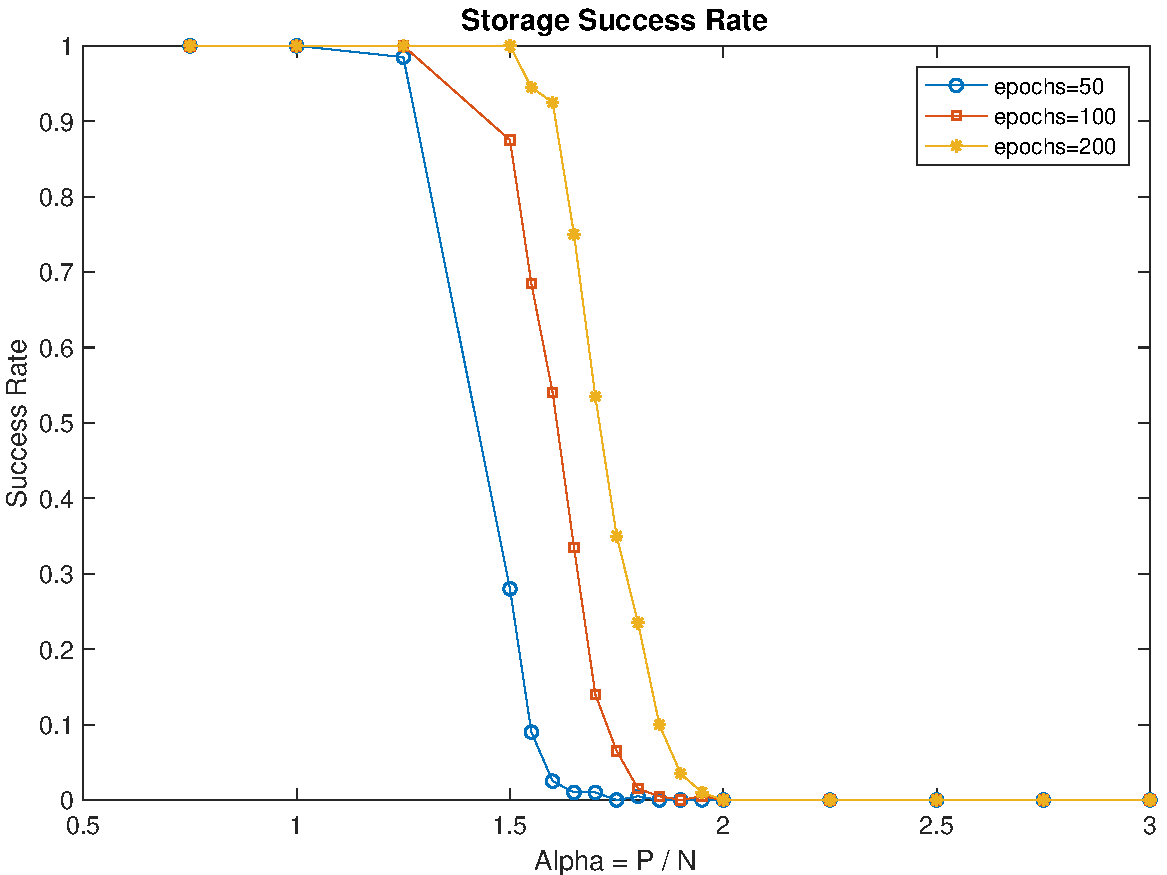
\includegraphics[width=\columnwidth]{figures/multiple_epochs}
    \caption{Storage success rate of a Rosenblatt perceptron as a function of $\alpha = P / N$ for different values of $n_{max}$.}
	\label{fig:multiple_epochs}
\end{figure}

The difference between the theoretical value and the experimental one are mainly due to the limited number of training iterations.
\cref{fig:multiple_epochs} gives an experimental proof of this statement:
for a very small number of iterations (eg. $n_{max} = 10$), the step is close to $\alpha = 1$, while for higher values of iterations the step moves closer and closer to the theoretical value $\alpha = 2$ found with \cref{eq:prob-lin-sep-alpha}.
The theoretical result still remains far from the practical one because of the limited size of input's dimension $N$.

\subsection{Number of Dimensions}
\label{subsec:dimensions}
\begin{figure}[t]
	\centering
	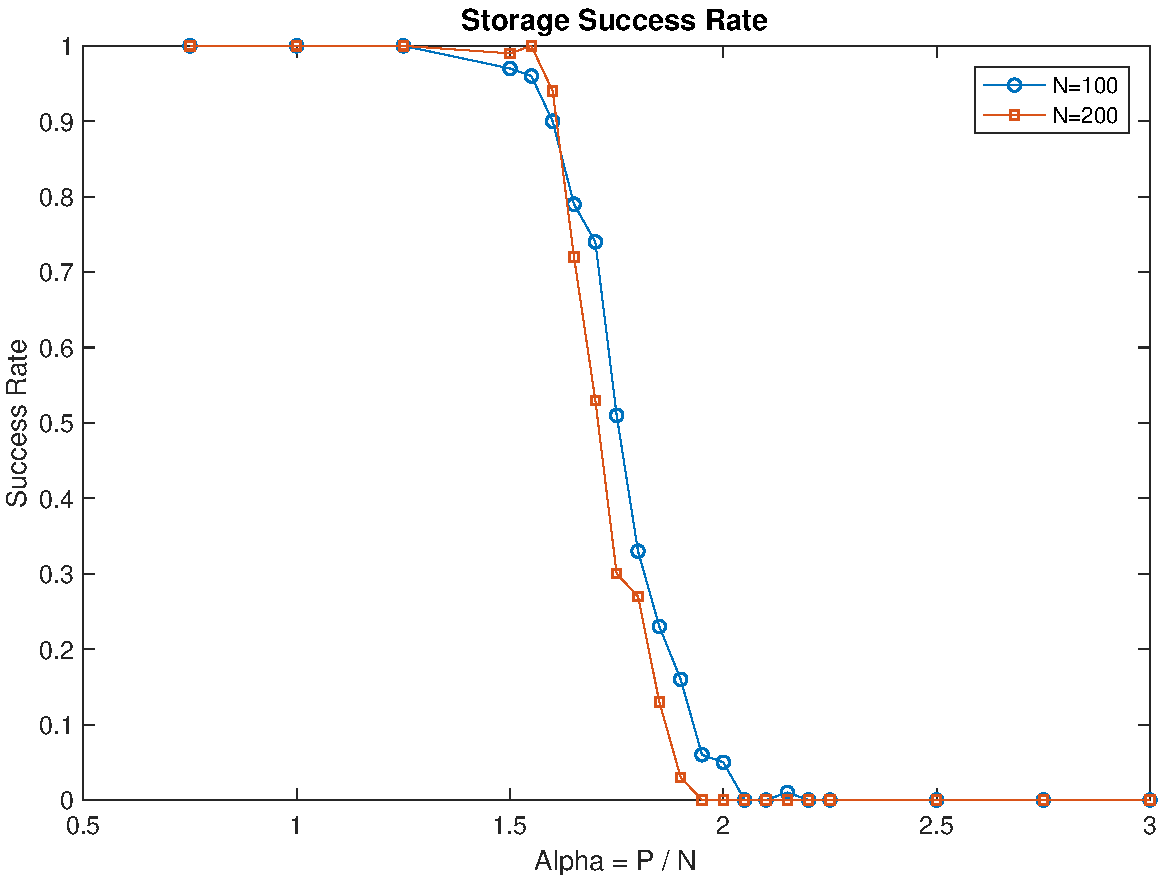
\includegraphics[width=\columnwidth]{figures/multiple_n}
    \caption{Storage success rate of a Rosenblatt perceptron as a function of $\alpha = P / N$ for different values of $N$.}
	\label{fig:multiple_n}
\end{figure}
The theoretical results are valid for $N \to \infty$.
However, real datasets have a limited number of features.
\cref{fig:multiple_n} shows the behaviour of the perceptron for different values of $N$.
For high values of $N$, the shape of the success rate $Q_{l.s.}$ as a function of $\alpha$ is similar to a step function.
For small values of $N$, the function looks like a smoothed step function:
the smaller $N$ is, the higher is the smoothing.

\subsection{Weight Update Criterion}
\label{subsec:c}
\begin{figure}[t]
	\centering
	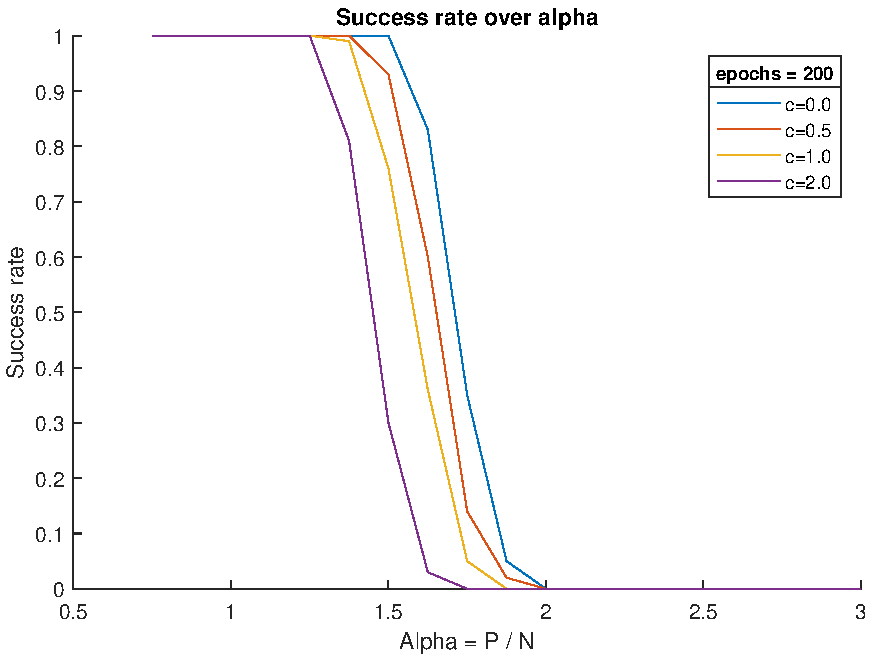
\includegraphics[width=\columnwidth]{figures/bonus_2_c}
    \caption{Storage success rate of a Rosenblatt perceptron as a function of $\alpha = P / N$ for different values of $c$.}
	\label{fig:multiple_c}
\end{figure}
\cref{fig:multiple_c} shows the effect of changing the values of $c$ in the training procedure of the perceptron.
For higher values of $c$, the curve is shifted to the left.
Since an example $\xi^\mu$ is considered correctly classified only when its local potential is greater than $c$ ($E = \mathsf{\bm{w}} \cdot \xi^\mu S^\mu > c$), the potential only depends on $\mathsf{\bm{w}}$ for a fixed $\xi^\mu$ and the update of $\mathsf{\bm{w}}$ is fixed for a given wrong classified example, the perceptron will need a higher number of updates to increase the norm of $\mathsf{\bm{w}}$ and make the local potentials higher than a threshold $c > 0$.
Formally, we can show that the value of $c > 0$ is irrelevant (provided the perceptron is trained long enough):
\begin{equation*}
	\mathsf{\bm{w}}_1 : \{E_1^\mu \geq c\}_{\mu = 1}^{P} \Leftrightarrow \mathsf{\bm{w}}_2 = \lambda \mathsf{\bm{w}}_1 : \{E_2^\mu \geq c\}_{\mu = 1}^{P}, \lambda > 0
\end{equation*}

\begin{figure}[t]
	\centering
	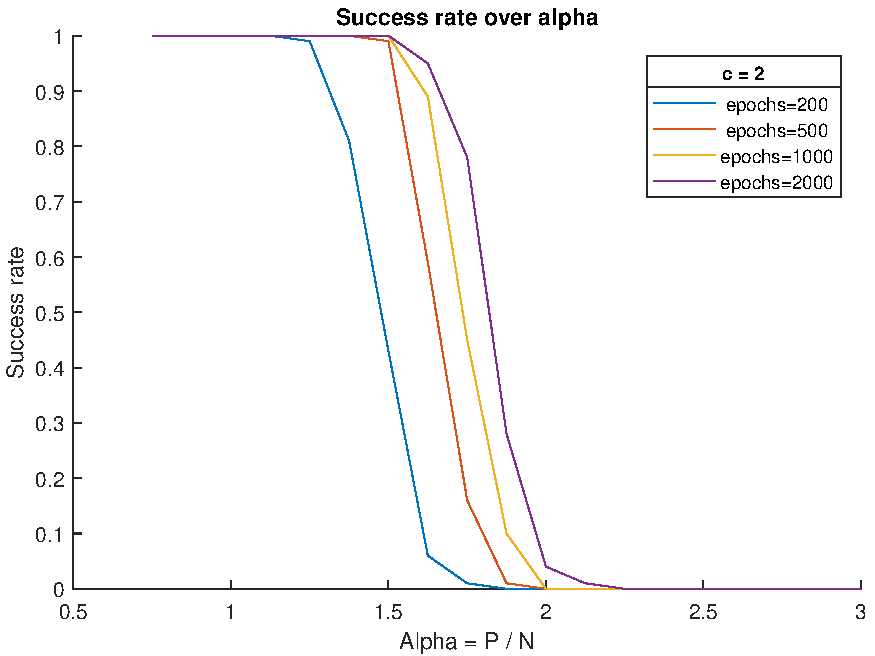
\includegraphics[width=\columnwidth]{figures/bonus_2_epoch}
    \caption{Storage success rate of a Rosenblatt perceptron as a function of $\alpha = P / N$ for different numbers of iterations with fixed value of $c=2$.}
	\label{fig:fixed_c_multiple_epoch}
\end{figure}
To give an empirical proof of this, we fix the value of $c$ and train the perceptron for different number of iterations $n_{max}$.
We expect to see the curve shifted to the left for small $n_{max}$, and approximate a step function centered in $\alpha = 2$ for big $n_{max}$.
\cref{fig:fixed_c_multiple_epoch} shows that the results of the experiment confirm our hypothesis.

\begin{figure}[t]
	\centering
	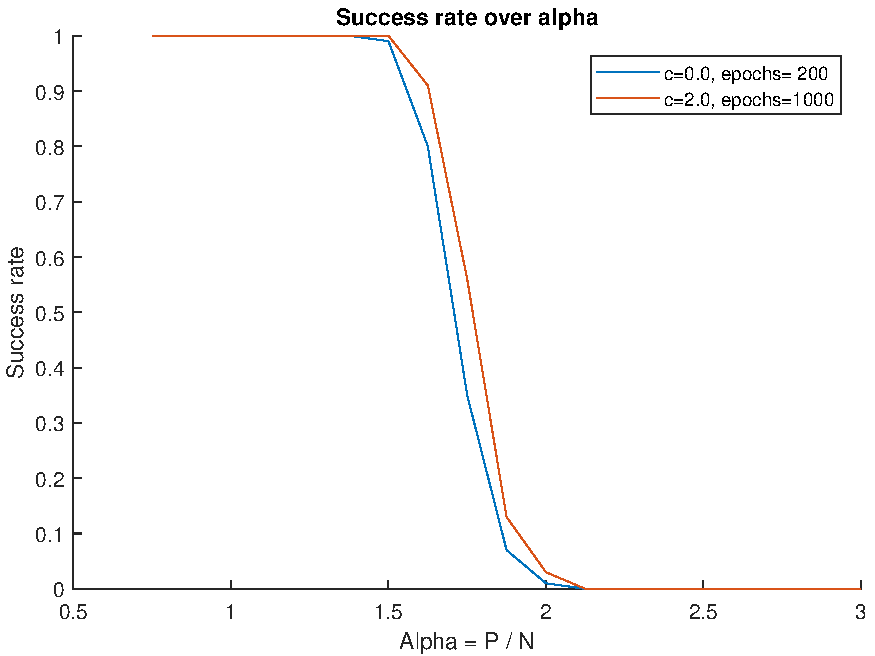
\includegraphics[width=\columnwidth]{figures/bonus_2_c_epoch}
    \caption{Storage success rate of a Rosenblatt perceptron as a function of $\alpha = P / N$ for different numbers of iterations and $c$.}
	\label{fig:multiple_c_multiple_epoch}
\end{figure}
\cref{fig:multiple_c_multiple_epoch} compares the curves for $c = 0$ and $c = 2.0$ for different values of $n_{max}$:
by increasing $n_{max}$, the curve is ``pushed'' towards the right, contrasting the effect of the increased value of $c$.
We can somehow see $c$ as a simple version of the learning rate that is used in more complex neural networks: it ``regulates'' the speed of the training.

\subsection{Inhomogeneous Hyperplanes}
\label{subsec:homogeneous}
\begin{figure}[t]
	\centering
	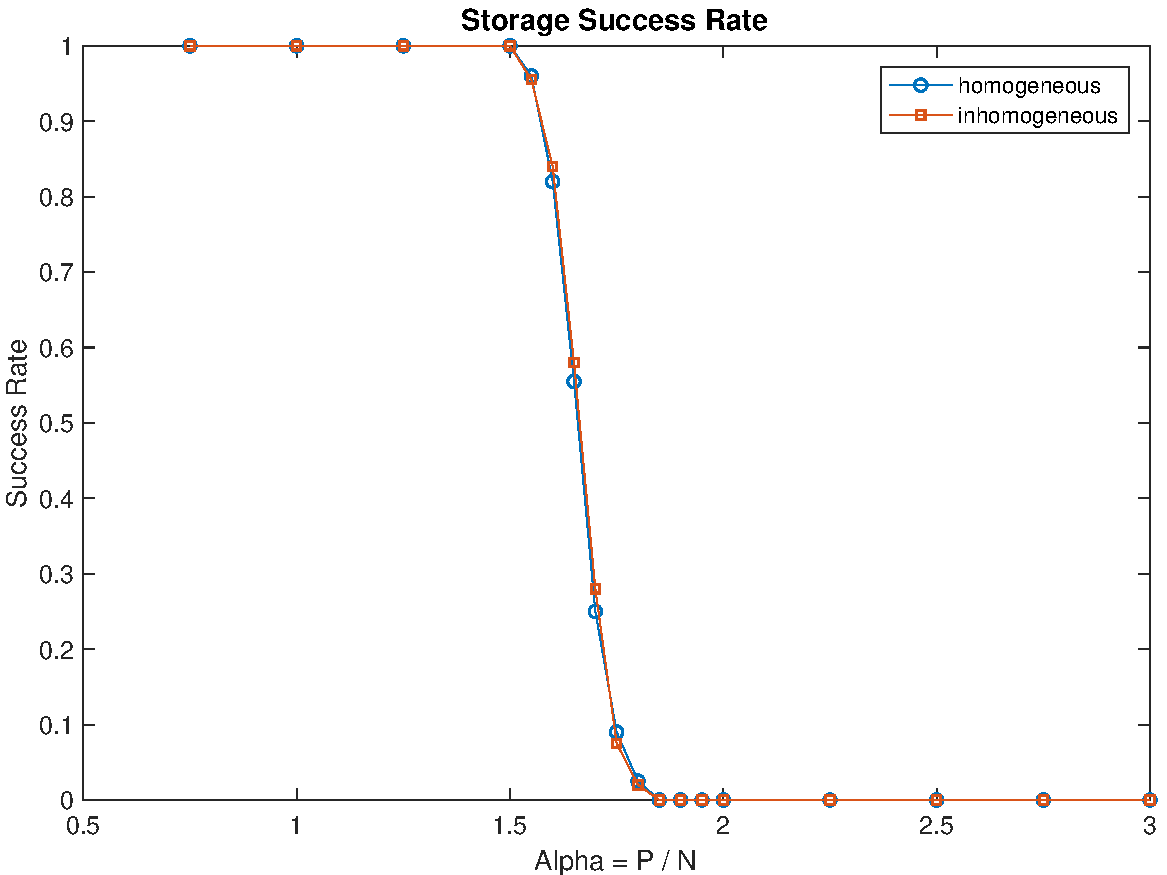
\includegraphics[width=\columnwidth]{figures/homogeneous}
    \caption{Storage success rate of a Rosenblatt perceptron and its inhomogeneous version for $N = 500$ as a function of $\alpha = P / N$.}
	\label{fig:homogeneous}
\end{figure}
We run an experiment to verify the behaviour of $Q_{l.s.}$ by allowing inhomogeneous hyperplanes:
we train both a normal and modified perceptron for $N = 500$.
\cref{fig:homogeneous} shows the results of the experiment.
As expected, the success rate $Q_{l.s.}$ of the inhomogeneous perceptron is slightly higher than homogeneous one.
However, the difference is not significant, since data points follow a normal distribution $\xi^\mu_j \sim \mathcal{N}(0,\,1)$ and are therefore distributed around the origin.

The problem of finding an inhomogeneously solution in $R^{N}$ can be solved by finding a homogeneously solution in $R^{N + 1}$.
In a second experiment, we compare the success rate $Q_{l.s.}$ of an inhomogeneous perceptron for $N = 500$ with an homogeneous perceptron for $N = 501$.
\cref{fig:homogeneous_n_n1} shows the result of this experiment.
As expected, the success rates for the $2$ perceptrons are very close to each other.

\begin{figure}[t]
	\centering
	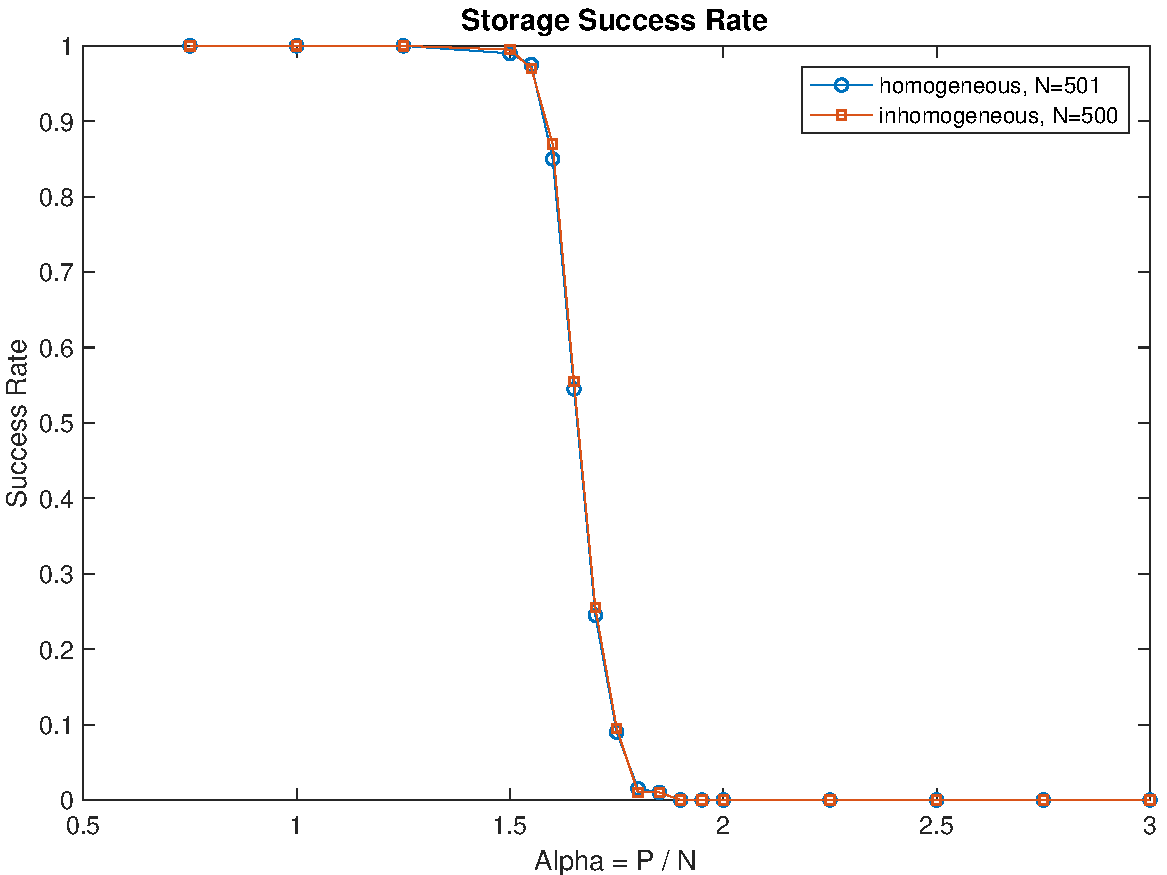
\includegraphics[width=\columnwidth]{figures/homogeneous_n_n1}
    \caption{Storage success rate of a homogeneous Rosenblatt perceptron for $N = 501$ and its inhomogeneous version for $N = 500$ as a function of $\alpha = P / N$.}
	\label{fig:homogeneous_n_n1}
\end{figure}

\section{Conclusion}
\label{sec:conclusion}

Stochastic Gradient Descent is an effective algorithm to learn the parameters of a feed-forward neural network.
The algorithm is iterative and takes as an input the number of iterations and a learning rate:
it is important to choose an appropriate value for both these parameters.
If the number of iterations is too small, the algorithms does not manage to learn the optimal parameters for the network;
if the number is too big, the model may overfit the training data and have bad performances on new data.
Similarly, if the learning rate is too small, the training may take too long or even stuck in local minima;
if it is too big, the updates may be too big and the model may never reach the optimal weights.

In general, it is difficult to choose the appropriate learning rate.
In some cases it may be effective to used a time-dependent one:
for example, one may set a big learning rate at the beginning and then reduce it to make the network converge easier.
We discussed some possible strategies and their effect on our regression problem.
However, a complete discussion of the possible learning rate policies is outside the scope of this document.


\bibliographystyle{IEEEtran}
\bibliography{references}

% \section{Appendix: \LaTeX\xspace Tips}

\subsection{Cross References}
\label{sec:cross-ref}

Cross references are an easy way to point a reader to certain parts of the text.
For figures, tables, and equations, they are a must.
Use the \verb|\cref| command to make references to a label.
For example, if you use \verb|\label{eq:newton-second}| to label the following formula
\begin{equation}
	\vec{F} = m\vec{a}\label{eq:newton-second}
\end{equation}
you can than refer to that in the text using \verb|\cref{eq:newton-second}|.
Example: The formula in \cref{eq:newton-second} is known as Newton's second law of motion.

\subsection{Figures}

A picture says more than a thousand words.
Use \texttt{jpeg} files for photos, use \texttt{png} for screenshots, use \texttt{pdf} for everything else.
Make sure to include all text required to get a (cursory) understanding of the figure in its caption; it is no problem to have a caption spanning five lines.
Do not put a second caption in the figure itself.
For closely related content, consider using subfigures.
Draw figures yourself, but acknowledge all sources.
Check font sizes to make sure the figure is neither unreadably small nor overly big.
For example, \cref{fig:bad,fig:good} show how voltage changes over time in a bad and in a good way, respectively.
\Cref{fig:bad} is bad because you cannot read the labels on the axis, and moreover the units are missing.
What is time measured in? Seconds? Milliseconds? And voltage? Volts? Millivolts? Kilovolts?
In contrast, \cref{fig:good} is clear and easy to read.

A warm suggestion: \textbf{DO NOT} fall into the temptation of using Excel (or similar stuff) to process your data and plot your graphs.
First, it is highly inefficient: if you need to re-plot your graphs (or change the way you perform data processing) you will need to \textbf{manually change all of them!}
Second, Excel-like plots are most of the time unreadable (and ugly), and they are not suited for presenting scientific results.
Use scripts and scientific tools to process and plot your data.
For example you might use \texttt{python} with \texttt{mathplotlib}\footnote{\url{http://matplotlib.org/}}, or the \texttt{R} statistical framework\footnote{Some basic examples at \url{http://flowingdata.com/2012/12/17/getting-started-with-charts-in-r/}}, or \texttt{gnuplot}, or MatLab.

\begin{figure}[t]%
	\centering
	\subfloat[bad figure]{\label{fig:bad}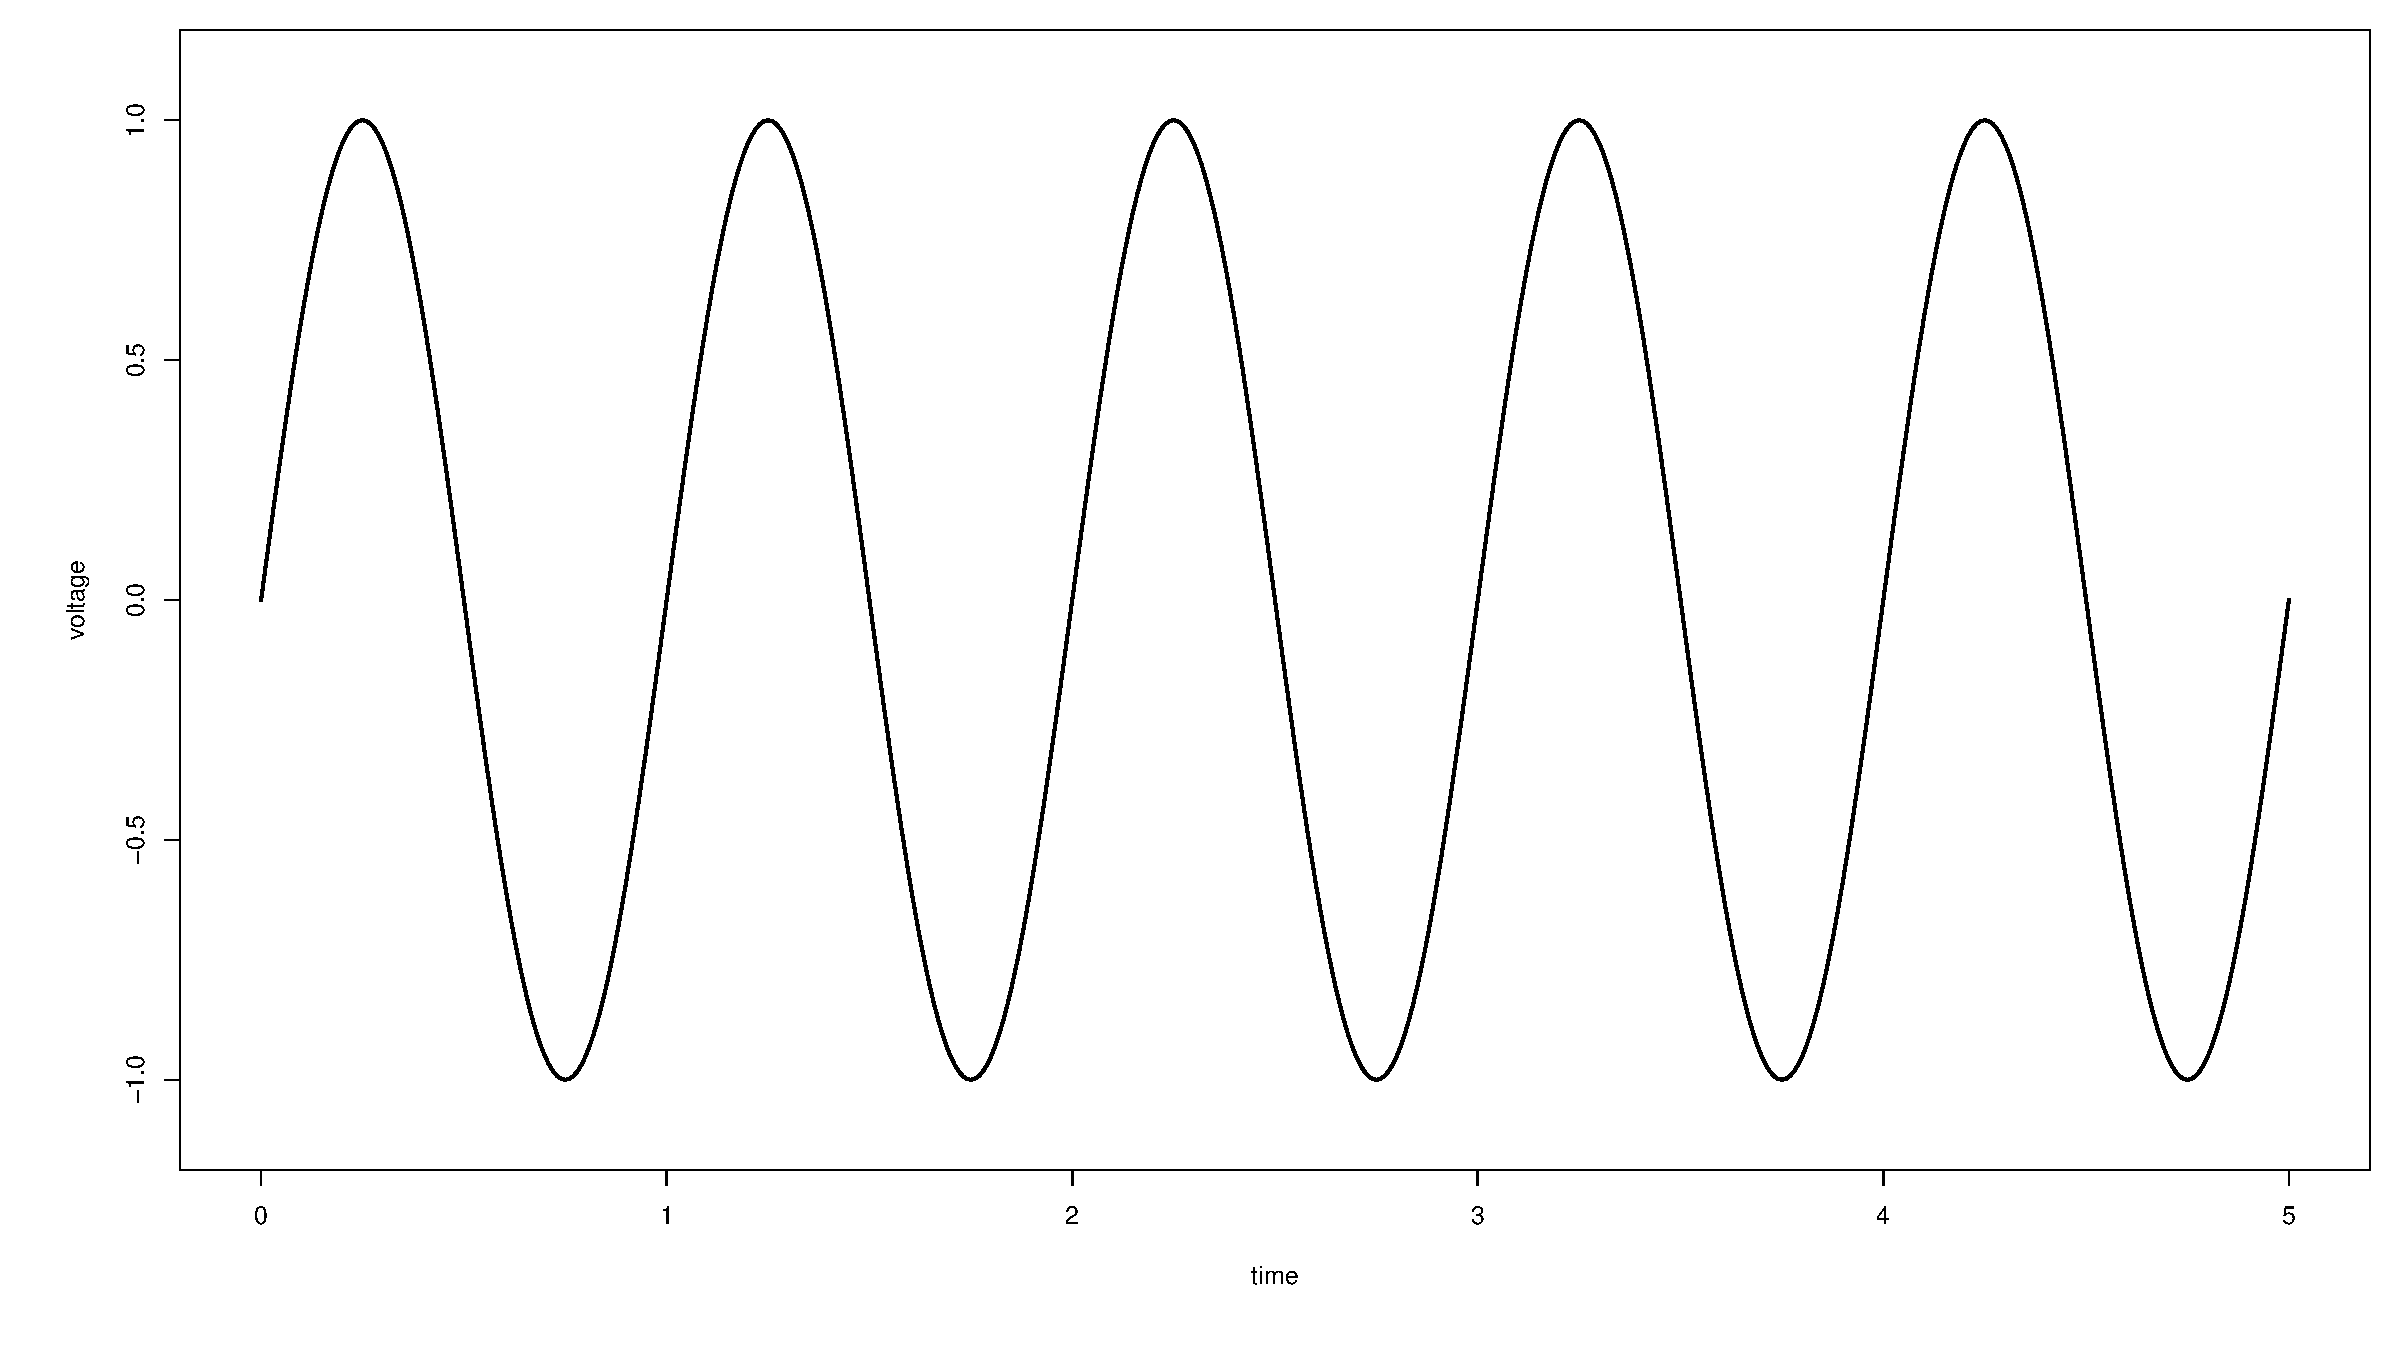
\includegraphics[width=\columnwidth]{figures/bad}}\\%
	\subfloat[good figure]{\label{fig:good}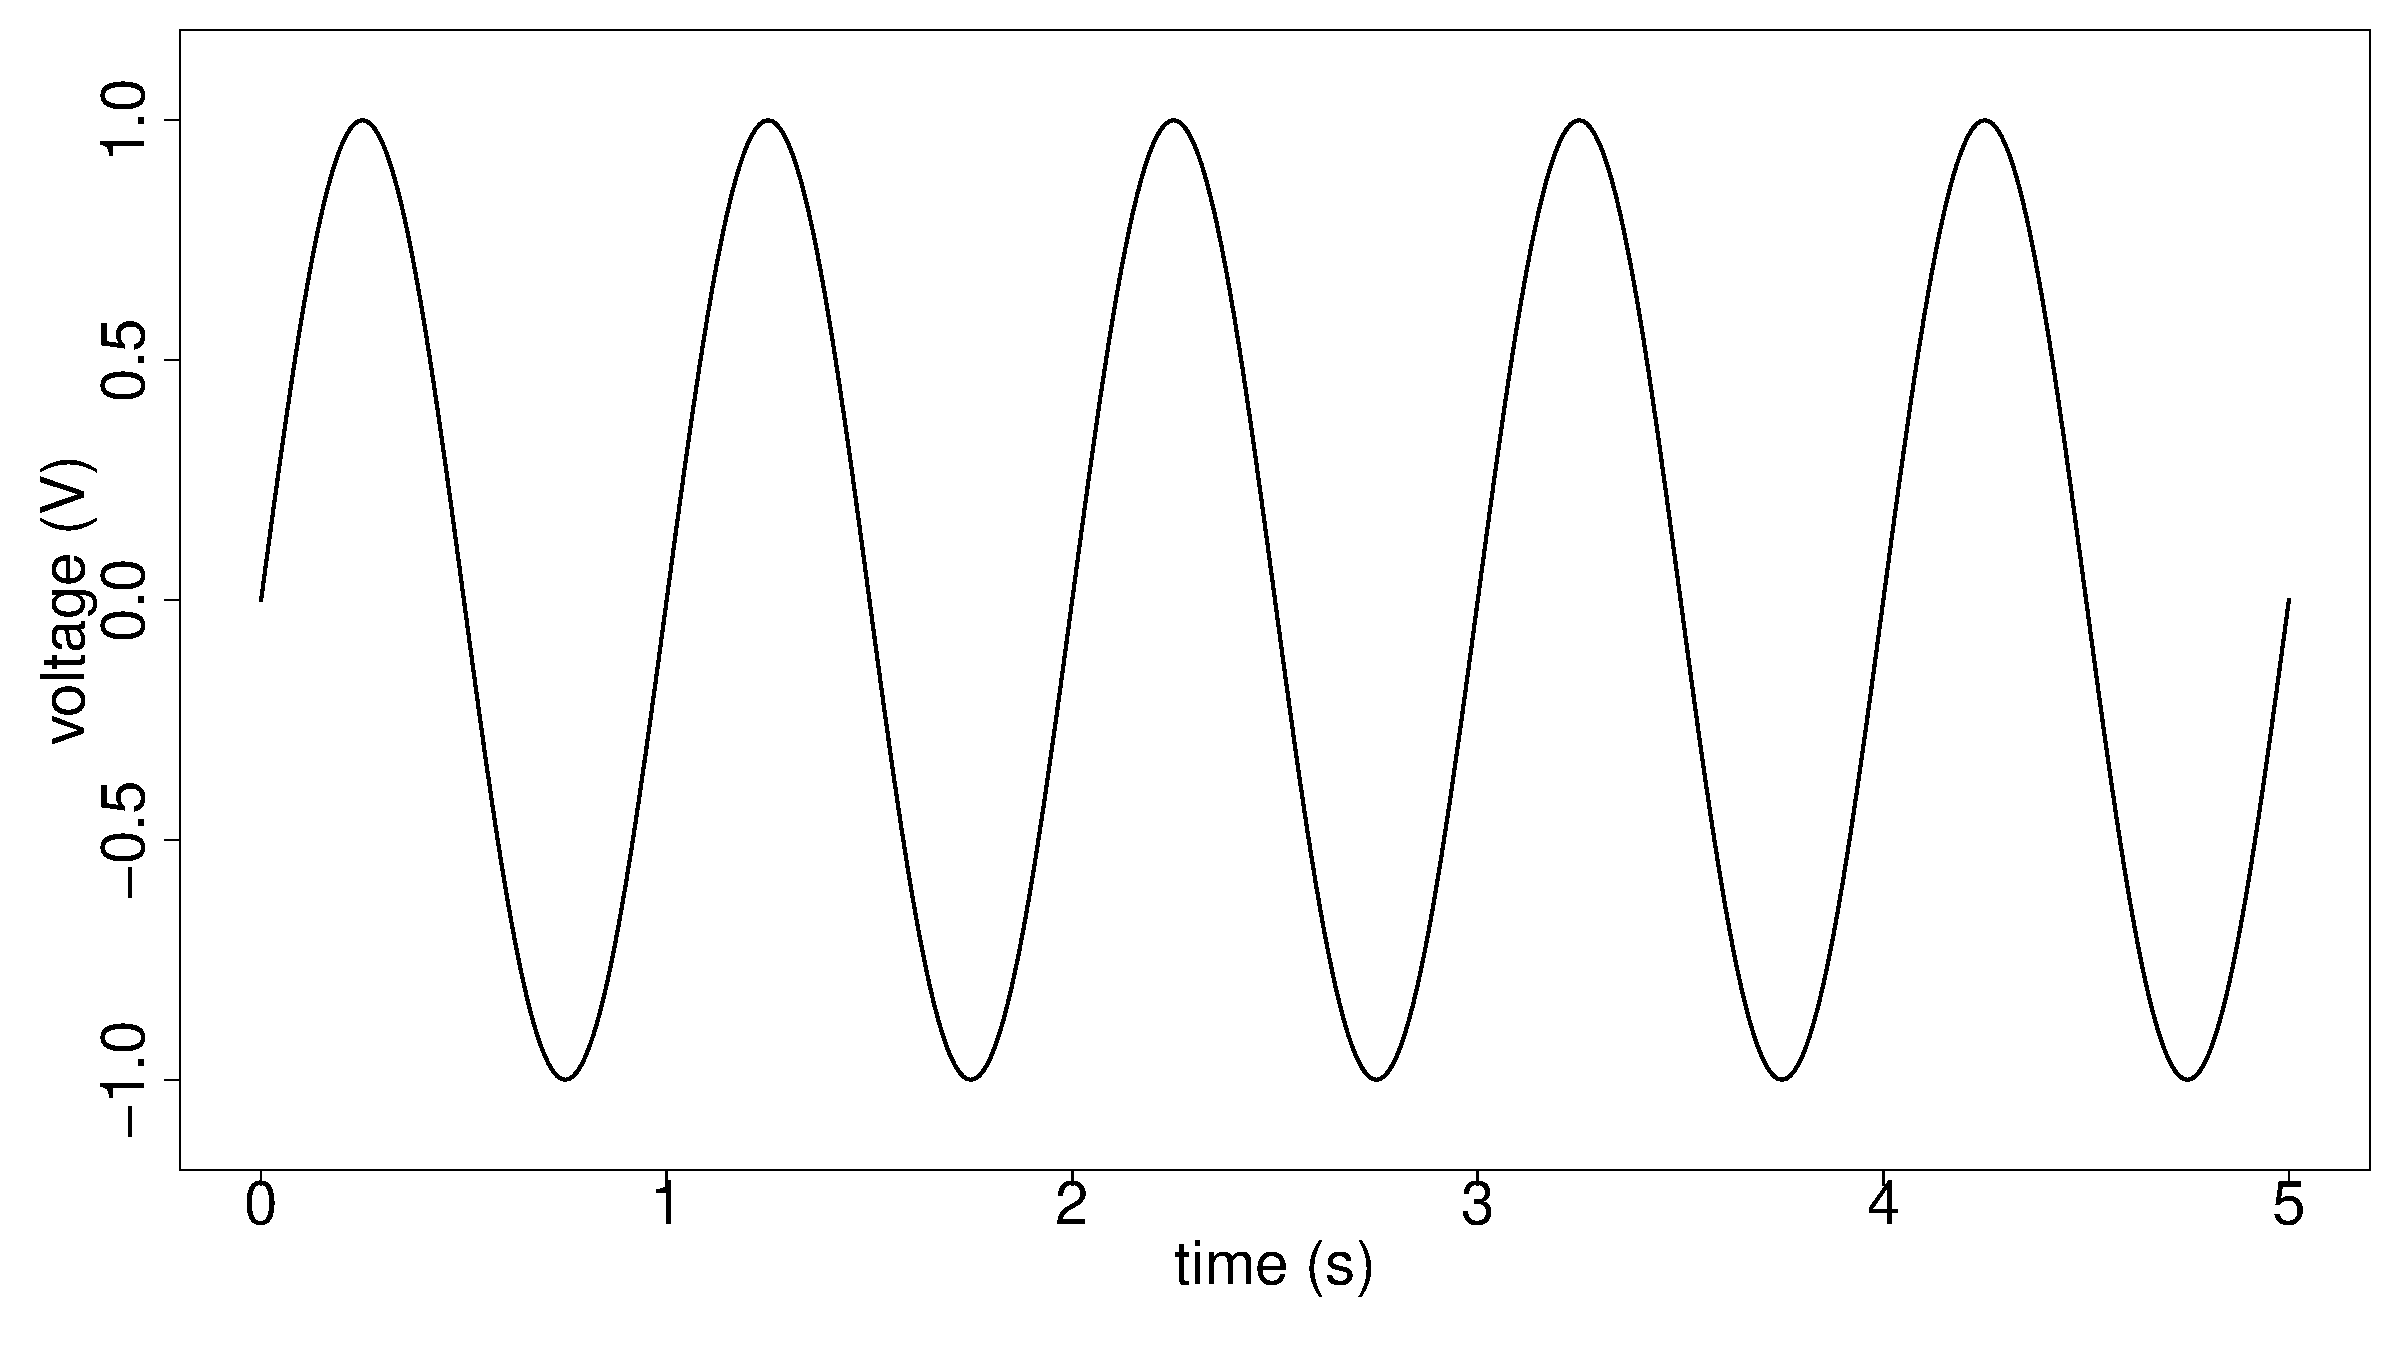
\includegraphics[width=\columnwidth]{figures/good}}
	\caption{A bad and a good representation of voltage over time.}%
	\label{fig:figures}%
\end{figure}

\subsection{Tables}

\begin{table}
	\centering
	\caption{Short table}
	\label{tab:shorttable}
	\begin{tabular}{llr}
		\toprule
		left aligned & same here & right aligned \\
		\midrule
		1 & 2 & 3 \\
		4 & 5 & 6 \\
		7 & 8 & 9 \\
		\bottomrule
	\end{tabular}
\end{table}

Use short tables, e.g., \cref{tab:shorttable} to give a brief overview of related information.
Tables are good, for example, to list your simulation parameters.

\subsection{Math}

\LaTeX's most famous feature is math typesetting.
You might need formulas for this assignment, so be sure to exploit all the power of this feature.
\begin{align}
sd_{max} &=
	\max\left(
		(t_{i+1} - t_i)
			: \zeta(t_i) < 1, i \in [0, |T|-1]
	\right)
,\\
\psi_{sd}(t) &=
	\begin{cases}
		\dfrac{\Delta t_{sd}}{sd_{max}}
			& \text{if $sd_{max} > 0$}, \\
		1
			& \text{if $sd_{max} = 0$},
	\end{cases}
\\
\zeta_{sd}(t) &= 
	\frac{
		\psi_{sd} - cl_{sd}
	}{
		c_{sd} - cl_{sd}
	}
.
\end{align}

The \emph{User's Guide for the amsmath Package}\footnote{\url{http://mirrors.ctan.org/macros/latex/required/amslatex/math/amsldoc.pdf}}, provided by the American Mathematical Society, has a comprehensive overview of best practices for typesetting mathematical content.

\subsection{Units}

Numbers with units should be set using the \verb|\SI| command, which enforces consistency throughout the text.
If you write units by your own, you will get inconsistent results: Different font faces when using text or math mode (e.g, 10 km/h versus $10 km/h$), or spacings (e.g., 10 km/h versus 10km/h), or conventions (e.g., 10 km/h versus 10 kmph).

For example: The measurements show that the car was accelerating at \SI{5}{\meter\per\second\squared} until it reached its final speed of \SI{100}{\kilo\meter\per\hour}.
Units only can be typeset using \verb|\si|; longer unitless numbers or ranges can be typeset using the \verb|\num| and \verb|\numrange| commands, respectively: The number \num{12345678} lies in the range of \numrange{10000000}{20000000}.
\Cref{tab:si-in-tables} gives an example of how to typeset numbers and units in tables.

\begin{table}
	\centering
	\caption{EMIT factors for a category 9 vehicle}
	\label{tab:si-in-tables}
	\begin{tabular}{l>{\raggedright}p{4cm}S[table-text-alignment=left,table-format=1.4e-1]s}
	\toprule
		\multicolumn{2}{l}{factor} & \multicolumn{1}{l}{value} & \multicolumn{1}{c}{unit} \\
	\midrule
		$M$ & vehicle mass & 1.3250e+3 & \kilo\gram \\
		$g$ & gravitational constant & 9.81 & \metre\per\second\squared \\
		$\vartheta$ & road grade & 0 & \degree \\
		$\alpha$ & & 1.1100 & \gram\per\second \\
		$\delta$ & & 1.9800e-6 & \gram\per\meter\cubed\second\squared \\
	\bottomrule
	\end{tabular}
\end{table}

%\section{Algorithms}
%
%Use algorithms to explain what would be too hard to express in the text body of your thesis.
%
%For example: Based on the periodically transmitted \texttt{hello} messages, the joining node gets information about its physical neighbors and their adjacent nodes.
%\Cref{alg:H_hello} depicts the handling of \texttt{hello} messages.
%
%\begin{algorithm}
%\begin{algorithmic}[1]
%\REQUIRE Locally stored state of all neighbors in set $N$
%\ENSURE Maintain neighbor set $N$ and set virtual address
%\STATE Receive neighbor information from node $N_i$
%\IF {$N_i \notin N$}
%	\STATE $N \gets N_i$
%\ELSE
%	\STATE Update $N_i \in N$
%\ENDIF
%\IF {$P==-1$ AND (Time() $-$ OldTime) $> T_{ps}$}
%	\STATE OldTime $\gets$ Time()
%	\STATE SetMyPosition()
%\ENDIF
%\end{algorithmic}
%\caption{Handle \texttt{hello} messages}
%\label{alg:H_hello}
%\end{algorithm}


%\section{Program Code}
%
%Program code should be omitted.
%What your programs do will already be explained in text form or, if needed, in algorithmic form.
%If including source code is absolutely necessary, it should be typeset as seen in \cref{lst:code}.
%
%\begin{lstlisting}[style=txt,caption=Sample application,label=lst:code]{}
%APPLICATION("printU", 192, arg)
%{
%    // Set Priority
%    NutThreadSetPriority(16);
%    // main() loop
%    for (;;) {
%        putchar('U');
%        NutSleep(125);
%    }
%}
%\end{lstlisting}

\subsection{References}

If you want to cite something proved in another work, use citations.
Search for the \texttt{bibtex} entry of the article you want to cite on \textit{ieeexplore} or \textit{google scholar}.
Put your \texttt{bibtex} code into \texttt{references.bib} and cite them using the \verb|\cite| command.
For example: According to \cite{akyildiz2002survey}, $1 + 1 = 2$.
The entries you cite will \textbf{automatically} appear in your references.

When citing more than a few pages worth of text, point the reader to the specific part you are referring to in your citation, like so:~\cite[Table IV]{dietrich2009lifetime}.

Do not cite URLs. For pointing a reader to interesting websites, use footnotes.

\subsection{Abbreviations}

Abbreviations should be explained when first used.
Latex helps by providing an \verb|\ac| command that will automatically expand an abbreviation on first use.

Example: \acp{MANET} have been frequently used as examples for the development of \ac{WSN} applications.
The literature provides hundreds different proposals of routing protocols for \acp{MANET}.
\subsection{Tips for Compiling your Latex Document}

Manually compiling your Latex document every time you make a change is terribly annoying.
Latex comes with a script which monitors your files and automatically re-compiles your document whenever a change in the file occurs.
If you change your text, you substitute a picture, or change your references, the script will re-build the pdf.

To use \texttt{latexmk}, first create (or edit) the \texttt{.latexmkrc} file in your home folder, independently from the OS (Linux, OS X, or Windows).
Inside the file put the following:

{\footnotesize
\begin{verbatim}
$pdflatex = 'pdflatex -interaction=nonstopmode';
\end{verbatim}
}

This will avoid \texttt{pdflatex} to stop in case of errors.
Then add the following (depending on your operating system and your pdf viewer).

On Linux

{\footnotesize
\begin{verbatim}
	$pdf_previewer = "start evince 2>/dev/null";
\end{verbatim}
}
On Mac OS X

{\footnotesize
\begin{verbatim}
	$pdf_previewer = "open ";
\end{verbatim}
}
On Windows

{\footnotesize
\begin{verbatim}
	$pdf_previewer = 'start "c:/Program Files\
	    /SumatraPDF (x86)/SumatraPDF.exe" %O %S';
\end{verbatim}
}

Then open your terminal, \verb|cd| into the folder where you have your latex document, and type

{\footnotesize
\begin{verbatim}
	latexmk -pdf -pvc <your-document-name.tex>
\end{verbatim}
}

On Windows you might need to type \verb|latexmk.exe|.
The script will compile your pdf and open the viewer when done.
If you make any change to your document and save it, you will see the script re-compiling the pdf.
The viewer should also automatically refresh the pdf.

\subsection{Concluding Remarks}

When working with latex, remember that this tool has a computer-science-like philosophy.
Everything is done \textbf{automatically}.
If you need to do something manually, you are doing something wrong!
You just want to write your text and let your computer do all the boring stuff (numbering pictures, link cross-references, list bibliography entries, align equations, \dots).
Remember to work smarter, not harder!
If you have troubles you cannot solve by browsing through the Internet, write us.

Good luck with your work!


\end{document}
